\documentclass[UTF8]{ctexart}

\usepackage{subfiles}  

%下面的语句, 引入你的头部设置文件
\usepackage{C:/phpStorm_proj/02_myself_ID_EGO/+100_latex_all_math_sel/myPreamble} 
%必须是绝对路径,才能让各个tex在单独编译时使用到

\title{向量组的线性相关性}


%---------------------------------


\begin{document}
	\tableofcontents % 生成目录
	\date{} % 若不写这句, 则默认也会渲染出日期, 所以我们要手动赋空值
	\maketitle  %这行代码, 让你前面的 title, author, date生效
	
	\section{向量 vector}
	
	通常, 当你考虑``一个"向量时, 就把它看成是``箭头". \\
	当你考虑``多个"向量时, 就把它看成是``箭头终点"的那个点(point).\\
	
	\textbf{注意: 向量的值, 表示的是坐标轴的位置, 而不是该向量线段的长度(即不是`模"的概念).}\\
	
	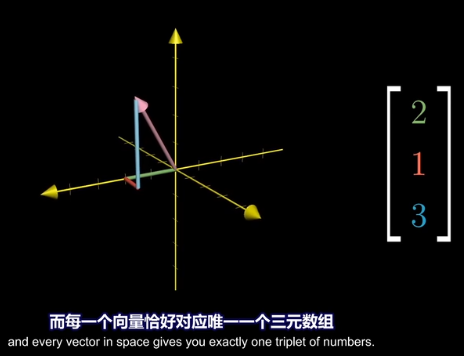
\includegraphics[width=0.4\textwidth]{img/0066.png}\\
	
	
	~\\
	\hrule
	~\\
	
	\section{向量的``数乘" : 系数k的作用, 是把向量伸缩 k倍}
	
	$2\left| \begin{array}{l}
		x\\
		y\\
	\end{array} \right|=\left| \begin{array}{l}
		2x\\
		2y\\
	\end{array} \right|
	$\\
	
	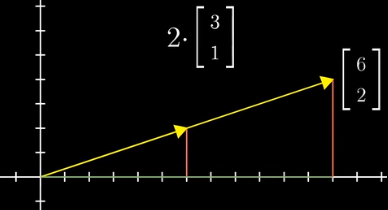
\includegraphics[width=0.4\textwidth]{img/0067.png}\\	
	
	系数k 为负数的话, 就是把向量朝``反方向"伸缩 k倍.
		
	~\\
	\hrule
	~\\
	
	\section{单位向量 : 基 basis}
	
	The \textbf{basis} of a vector space /is a set of linearly independent vectors /that span the full space.
	
	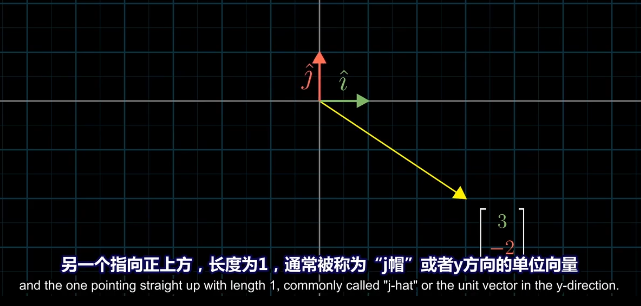
\includegraphics[width=0.6\textwidth]{img/0068.png}\\	
	
	$\left. \begin{array}{r}
		\hat{i} = 1\\
		\hat{j} = 1\\
	\end{array} \right\}$ ← 称为``单位向量"或``基"\\

事实上, 每当我们描述一个向量时, 它都依赖于我们正在使用的``基".\\

$\vec{v}=\left| \begin{array}{l}
	3\\
	-2\\
\end{array} \right|= 3 \hat{i} + (-2)\hat{j}$\\

	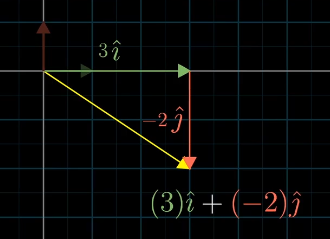
\includegraphics[width=0.3\textwidth]{img/0069.png}\\		
	
	向量的终点坐标, 其实就是系数倍的``基向量"的线性组合.
	
	~\\
	\hrule
	~\\
	
	\section{张成 span}
	
	the span of $\vec{v}$ and $\vec{w} $  /is the set of  all their linear combinations.\\	
	the set of all possible vectors /than you can reach /is called the span of those two vectors. ← 相当于``势力范围", 就是张成.\\
	
	
	两个斜率不同的向量(a,b), 自由伸缩, 它们的和(即a+b=c), 即新向量c的终点, 能遍及二维平面上的任何点处.\\
	
		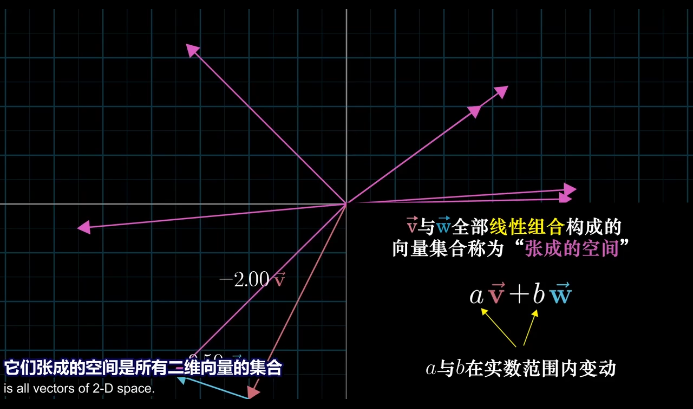
\includegraphics[width=0.6\textwidth]{img/0070.png}\\	
	
	但如果两个向量都是``零向量"的话, 它们的系数倍的和, 也永远被束缚在原点(0,0)了. $ k_1 \vec{0}  +  k_2 \vec{0}=0$ \\
	
	三维空间中, 两个斜率同的向量, 能``张成"出``过原点"的一个平面.\\	
			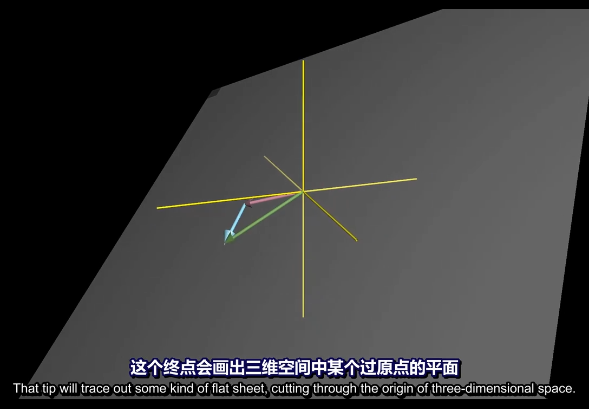
\includegraphics[width=0.4\textwidth]{img/0071.png}\\
			
	三维空间中, 三个斜率不同的向量, 它们的和, 能张成出三维空间中所有的地方. \\			
			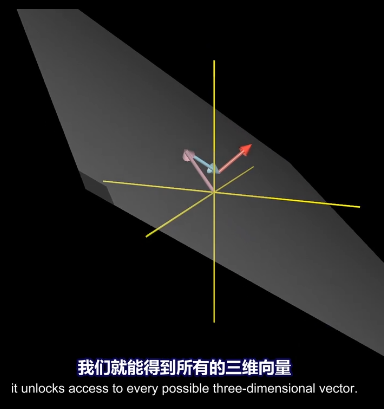
\includegraphics[width=0.4\textwidth]{img/0072.png}\\
	
	
	~\\
	\hrule
	~\\
	
	\section{向量的叉积(外积) : $\vec{v} \times \vec{w}$}
	
	向量的 叉积 (外积) exterior product 或  cross product
	
	
	
	\subsection{叉积(外积) 的几何意义 : (1)在二维空间中, 是由这两个向量围成的``平行四边形"的面积, 即是一个数值. (2)在三维空间中, 是一个垂直于这个``平行四边形"平面的``新向量".}
	
	【在二维空间中】: \\
	
	\textbf{几何意义上, 叉积, $\vec{v} \times \vec{w}$, 就是由这两个向量围成的``平行四边形"的面积.} \\	
	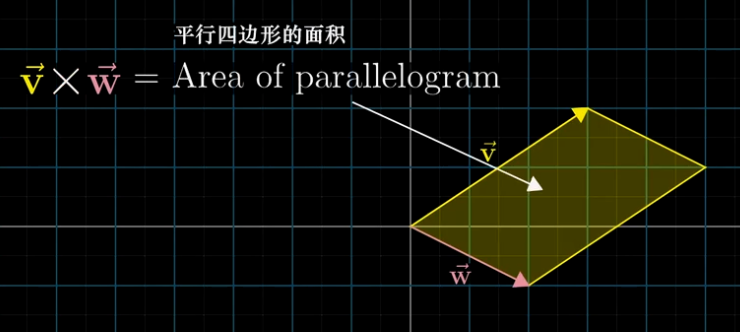
\includegraphics[width=0.5\textwidth]{img/0073.png}\\
	
	\textbf{注意: 顺序会对``叉积"有影响: 如果$\vec{v} \times \vec{w}$ 是正数, 则 $\vec{w} \times \vec{v}$ 就是负数. 即: 交换叉乘时的顺序, 值要变号.} \\
	
	之前说过, 行列式的值, 就是表示的是: 将基 $i \times j$ 的面积, 缩放多少倍.\\	
	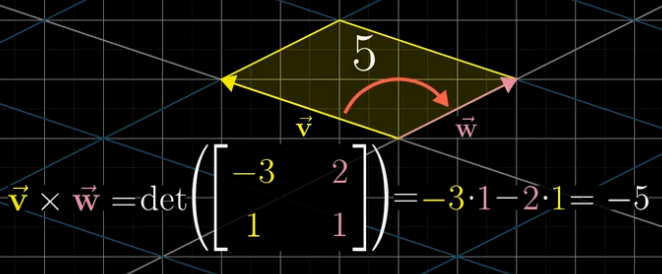
\includegraphics[width=0.5\textwidth]{img/0074.png}\\
		
	面积的概念, 也就证明了: $3(\vec{v} \times \vec{w}) = 3 \vec{v} \times \vec{w}$\\	
	把平行四边形其中的任一一条边, 延长3倍 , 变成 $3 \vec{v}$ 或  $3 \vec{w}$, 面积也就是 $= 3 (\vec{v} \times \vec{w})$ \\
	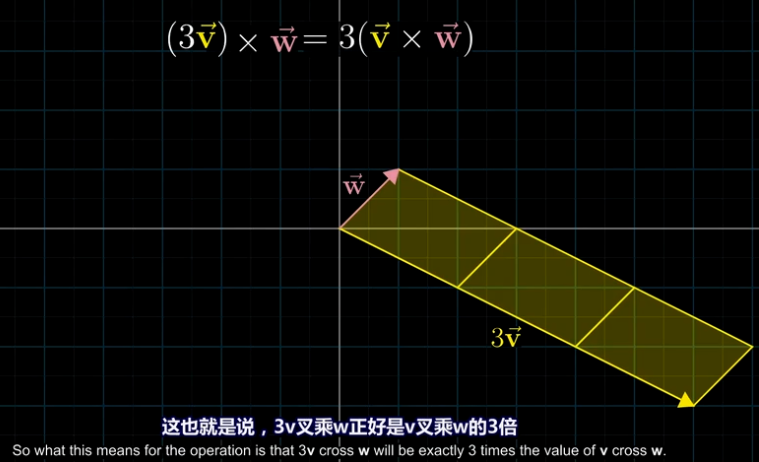
\includegraphics[width=0.5\textwidth]{img/0075.png}\\	
	
	
	
	
	【在三维空间中】:\\	
	其实, 真正的``叉积", 是通过两个三维向量, 来生成一个新的三维向量. \textbf{注意: 在三维空间中, 叉积的结果不是一个数, 而是一个向量!} \\
	
\begin{myEnvSample}
	如下面的图中所示, A,B两个箭头的向量的``叉积", 就是第三个向量C. 这个C向量, 始终与两个原点箭头(即A,B)正好为90度.  C向量箭头的长度, 就表示A,B向量的叉积, 它总是完全等于A,B所构成的平行四边形的面积.\\
	
		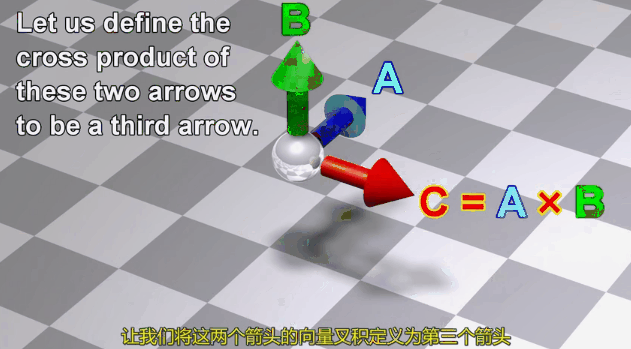
\includegraphics[width=0.4\textwidth]{img/0076.png}
		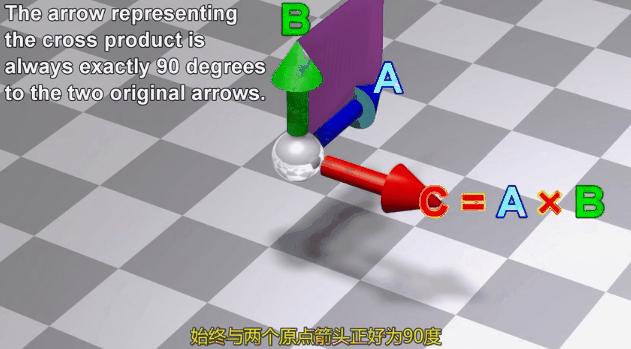
\includegraphics[width=0.4\textwidth]{img/0077.png}\\
		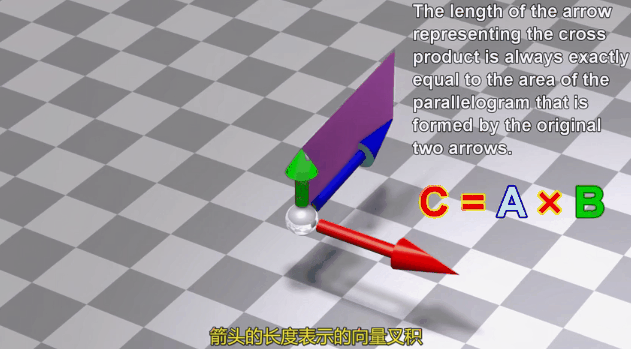
\includegraphics[width=0.4\textwidth]{img/0078.png}
		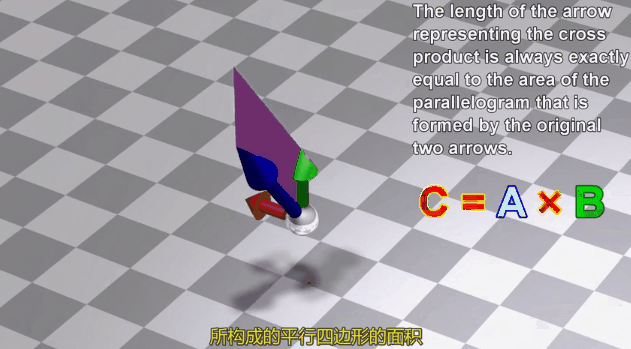
\includegraphics[width=0.4\textwidth]{img/0079.png}\\
	\end{myEnvSample}


	\begin{myEnvSample}
	又如: 假设$\vec{v} \times \vec{w} = 2.5$, 在三维空间中, 这两个向量构成一个平面(平行四边形). 它们的``叉积"构成一个新向量 $\vec{p}=2.5$, 它与``平行四边形"所在的面``垂直".\\
	
	
	
	
	
	\end{myEnvSample}


	
	
	
	
	
	
	% https://www.bilibili.com/video/BV1aW411Q7x1?p=20&vd_source=52c6cb2c1143f8e222795afbab2ab1b5
	% 3.11
	
	
	
	
		----------------
	
	\part{向量组, 及其线性组合}
	
	\part{向量组的线性相关性}
	
	\part{向量组的秩}
	
	\part{线性方程组的解的结构}
	
	\part{向量空间}
	

	
\end{document}